\section{Other vendors: arms GM, GM2, GM3 and V}\label{sec:gm3-v}

Arms GM, GM2, GM3 and V change the vendor. GM3, the only chain arm with a verdict, meets the
registered pooled bar, 46 of 80. In a post hoc split it misses at the discriminating cells,
11 of 43, where the modal output is the family argmax construction. In arm V ten of thirteen aliases fall below the floor, and
the three that clear it split, two anchoring at point estimate and one not. Arms GM, GM2 and
GM3 run against a second vendor's first-party API and vary the model family, with prompts
pinned, an output budget fixed and a provider logged per row. Arm V varies vendor and serving
class at once.

\textbf{Arms GM and GM2 returned no scoreable data, and both are reported.} One chain
registration fixes the definitions and predictions for all three GM arms. Each arm addresses
seven $N$ cells by twenty samples, over a floor of three valid samples per cell. The primary
prediction requires a mode match in at least 5 scoreable cells. The second requires a pooled
on-prediction rate of at least 30\%. The third requires the two-radius signature at order
$k^*$ in at least half of on-prediction samples. That signature is a grid radius $1/(2k^*)$
carrying a filler radius $(\sqrt{2} - 1)/(2k^*)$. The falsifier fires on a mode-match failure
in at least 4 scoreable cells. Arm GM addressed a gemini-flash-lite alias, part of it through
a routed path (Supplement~S2). It returned 20 valid of 140, UNDERPOWERED under both
accountings, and its falsifier fires under neither. Arm GM2 addressed the gemma family at a 4,096-token output budget, and returned 0 of
140 parseable. The cause is a budget confound, not a model result. The vendor API returns
deliberation on a separate channel, and the budget was spent there before any answer text. Arm
GM3 re-ran the design at 16,384 tokens. Of its 140 rows, 17 did not parse. Of the 123
that did, 80 are valid packings at $10^{-6}$.

\textbf{Arm GM3: the pooled bar is met and the discriminating cells are not.} Arm GM3 runs the
unconditioned-call protocol against gemma-4-26b through the vendor's first-party API. The
first-party key reached its quota, so 41 of the 140
rows were sampled through a routed path under an amendment committed before resumption, and
both accountings are reported.

The pooled prediction held. Of the 80 valid packings, 46 land within $2\times10^{-3}$ of the
value the closed form predicts. That clears the registered pooled bar. The 41 routed rows
carry 2 of the 80 valid packings. None of the 46 on-prediction are among them. First-party
rows alone
therefore give 46 of 78, and no verdict changes. A pooled rate cannot separate family search
from anchoring, because the two agree off the discriminating cells. The two cells where the anchor equals the family argmax
hold 35 of the 46 on-prediction packings. On the three scoreable discriminating cells, a
split read post hoc, the rate is 11 of 43, below the bar the pooled metric passes.

The cell-level bar was not met. The anchor is modal in 2 of 5 scoreable
cells, and Figure~\ref{fig:gm3anchoring} plots the per-cell modal sums against the
anchor. The falsifier did not fire either: three failures, short of its four. Bar
and falsifier together leave one to three failures unadjudicated, a registration design gap,
and the observed three fall in it. The two-radius signature also came in under its bar of half. Only 20 of 46 on-prediction
samples carry the exact decomposition. That bar cannot be met at a truncate cell, whose anchor carries one radius
and no filler. The 15 on-prediction samples at $N = 35$ are counted against a signature they
could not show.

\begin{figure}[t]
\centering
\begin{minipage}[c]{0.44\linewidth}
\centering
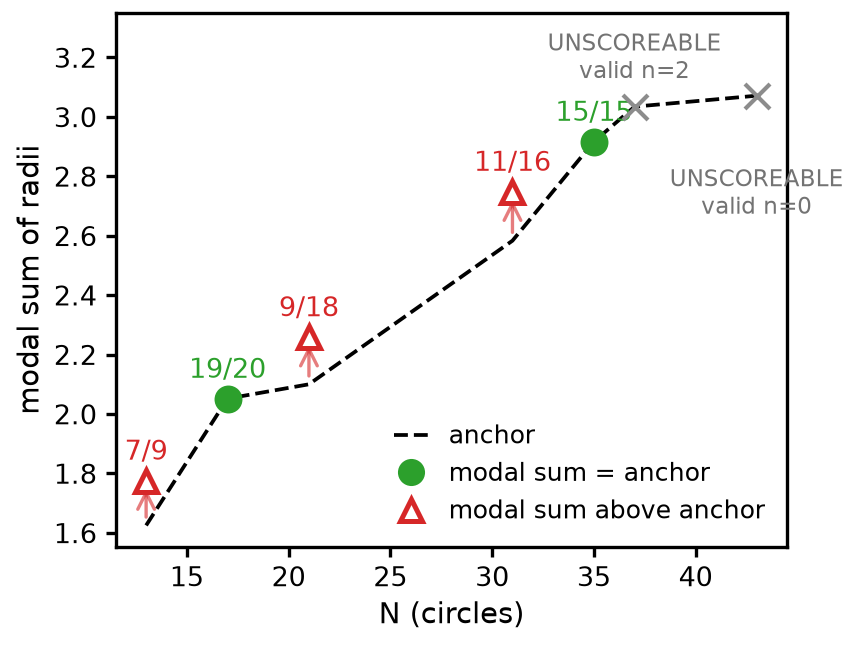
\includegraphics[width=\linewidth]{fig_gm3_anchoring.png}
\end{minipage}\hfill
\begin{minipage}[c]{0.53\linewidth}
\caption{\emph{Arm GM3 modal sums against the anchor.} Filled green circles
match the anchor (the dashed line is $V(k^*, m)$ at extend cells and $T(k^*, N)$ at
truncate cells), with frequencies annotated. Open red triangles miss, and every miss lands
above the anchor at the family argmax \emph{value}. The post hoc structural check in the
text, not this figure, establishes that these are also the family argmax \emph{construction}.
Grey crosses on the anchor line are the two UNSCOREABLE cells, with their valid counts.
Regenerates via \texttt{fig\_gm3\_anchoring.py}
from \texttt{arm\_gm3\_report.json}.}
\label{fig:gm3anchoring}
\end{minipage}
\end{figure}

\textbf{The misses are the family argmax construction (post hoc, disclosed).} The modal
output at every discriminating cell is the family argmax itself. A post hoc structural diagnostic finds all 27 of the 27 packings at the family
argmax value carrying its two-radius decomposition, at the $10^{-3}$ radius tolerance the
diagnostic uses. That
decomposition is the $(k^*{-}1)$ grid radius with the $(k^*{-}1)$ filler radius. The
registered signature test could not see this, because it tests radii against the predicted
order $k^*$. On the discriminating cells 27 of 43 valid packings are the family argmax
construction. That is 63\%, on a 48--76\% interval. Validity collapses at the two largest
cells, $N = 37$ and 43, which bounds where this model returns evaluable packings; both are
UNSCOREABLE under the registered rule. Clearance was re-read post hoc,
as for arm MU. Of the 80 valid packings, 79 are valid at $10^{-9}$. None clears the family
argmax under the rule of \S\ref{sec:method}. Twenty-nine of the 79 sit above it by at most
$5.3\times10^{-10}$, the rounding of a printed coordinate. The rest sit at or below
(Supplement~S4).

\textbf{Arm V: thirteen free-tier aliases.} Arm V sends the GM chain's prompt files
byte-identical at five cells, $N = 13$, 17, 31, 35 and 37. It draws five samples per model and
cell. The targets are free-tier aliases across seven attributed vendors. Three amendments,
each committed before the sampling it
governs, expanded the original three-alias design to thirteen aliases across two serving
paths. The last raised the output budget after hidden-reasoning truncation emptied three
models' replies.

Execution retried each invocation slot until content arrived, per the registered
transport-repair rule. The per-model floor of \S\ref{sec:method} is evaluated on registered
slots, so a slot with no row counts against it. Ten of thirteen aliases finished BELOW-FLOOR,
including all three originally registered aliases. One of them made 108 attempts across its 25
registered slots, none of them with content. The other three cleared the floor, and their
registered verdicts split.

V1 predicted at least 50\% of a model's valid outputs on-prediction, and V2 at most 10\% at
the family argmax. V2 is scored only at the discriminating cells, $N = 13$ and 31. In this
arm, \emph{transfer} denotes only the registered pooled-bar verdict. An alias must clear the
per-model floor and meet the V1 bar on its valid outputs pooled over five cells. Every transfer
verdict here rests on amendment-added aliases. All three were registered by amendment 2
(\texttt{arm\_v\_\bk{}preregistration\_\bk{}amendment2.md}, \texttt{d579797}).

\begin{center}
\footnotesize
\setlength{\tabcolsep}{3.5pt}
\begin{tabular}{@{}llcccc@{}}
\toprule
alias & vendor & valid & V1 on-prediction & V1 bar ($\ge$50\%) & \begin{tabular}[b]{@{}c@{}}V2 family argmax\\valid at discriminating cells\\(bar: $\le$10\%)\end{tabular} \\
\midrule
\texttt{north-mini-code} & Cohere & 12 & 8/12 [39--86\%] & \textbf{MET} (point est.) & 0/4 \textbf{HOLDS} \\
\texttt{gpt-oss-20b} & OpenAI & 18 & 11/18 [39--80\%] & \textbf{MET} (point est.) & 0/9 \textbf{HOLDS} \\
\texttt{gemma-4-31b-it} & Google & 15 & 0/15 = 0\% [0--20\%] & \textbf{NOT MET} & 0/3 \textbf{HOLDS} \\
\bottomrule
\end{tabular}

{\footnotesize Bracketed ranges are 95\% Wilson intervals on the rate they follow. V2 is
scored only at the discriminating cells. The registration labels a met V1 bar TRANSFERS and a
missed one DOES-NOT-TRANSFER; this table reports the bar outcome, in the sense
\S\ref{sec:gm3-v} defines. Both passing intervals span the 50\% bar.}
\end{center}


\textbf{Both passes are weaker than the percentages suggest.} The
bracketed Wilson 95\% intervals include the bar, so each verdict is a point-estimate pass.
And the pooled rate spans cells that cannot
discriminate anchoring from family search. Decomposing onto the discriminating cells gives 3
of 4 for the first alias. It gives 5 of 9 for the second. The arm's strongest reading, that these aliases behave
as the original family does, does not survive the template-shape null. That null is a proposer
picking uniformly at random among the admissible grid orders in $k^*{-}1$, $k^*$ and $k^*{+}1$,
one branch value each. It lands on-prediction one time in three at every cell but $N = 17$,
where one order overfills its interstices and the rate is one in two. Supplement~S5 derives it in
this paper's own terms and gives the exact tails, and this paper applies it post hoc
\citep{companion}. The pooled rates clear that null only because most of their cells cannot
discriminate. At the cells that can, neither pass separates from it. Arm GM3's
post hoc 11 of 43 at its discriminating cells does not separate from it either. V2 is a point-estimate
pass on 16 valid outputs at discriminating cells: 0 land on the family argmax, on per-alias
counts of 3, 4 and 9 whose Wilson intervals all include the 10\% bar. The same post hoc re-read over the three evaluable aliases
finds 45 valid at $10^{-6}$ and 39 at $10^{-9}$. None clears the argmax; eight of the 39
sit above it by $8.9\times10^{-16}$, float noise, and the rest sit at or below. The closest at
a discriminating cell
falls short of it by $2.5\times10^{-3}$ at $N = 31$ (Supplement~S4).

\textbf{Anchoring is not confined to the original family, and not universal.} Two further
vendors' models land the registered construction values at point estimates above the bar.
Through the chain's first-party API, gemma-4-26b emits the family argmax construction at
the discriminating cells. Through arm V's free-tier serving path, gemma-4-31b lands neither the
anchor nor the family argmax. Its valid packings are de-novo, unanchored and weak. Their per-cell bests run
0.88--1.85. The anchors at those cells run 1.63--3.03. Model variant and serving path
change together across this pair, so the boundary is located but not attributed.
